\documentclass[hyperref={pdfpagelabels=false}]{beamer}
\usepackage{color}
\usepackage{colortbl}
\usepackage{graphicx}
\pagestyle{empty}
\usepackage{wrapfig}

\definecolor{DarkGreen}{rgb}{0.17,0.60,0.25}
\definecolor{lightBlue}{rgb}{0.67,0.835,0.99}
\definecolor{brown}{rgb}{0.68,0.403,0.153}
\definecolor{Pink}{rgb}{1.,0.75,0.8}

\newcommand{\tc}{\textcolor}

\usepackage[utf8x]{inputenc}
\usepackage{default}

\begin{document}

%-------------------------------------------------------------------------------
% Title frame
%-------------------------------------------------------------------------------
\begin{frame}
\begin{center}

{\Large
Project Proposal\\
}
\bigskip
\bigskip

\textcolor{blue}
{\Large
Hadoop and Hive as scalable alternatives to DBMS business intelligence solutions
for Big Data
}

\bigskip
\bigskip

\textcolor{red}
{\large\em
Marissa Hollingsworth
}

\medskip

{\small
Department of Computer Science\\
College of Engineering\\
Boise State University
}

\end{center}
\end{frame}

%-------------------------------------------------------------------------------
% Big Data frame
%-------------------------------------------------------------------------------
\begin{frame}
\frametitle{\hspace{.35\textwidth} 
\includegraphics[height=.75in,
keepaspectratio=true]{./images/big-data.jpg}}

{\it A term applied to data sets whose size is beyond
the ability of commonly used software tools to capture, manage, and process the
data within a tolerable elapsed time.}\hspace{1in}-Wikipedia\\
\bigskip
\pause
\begin{itemize}
 \item {\it ``More data usually beats better algorithms.''}\\
	\hspace{.6\textwidth}-Anand Rajaraman
  \pause
 \item High-cost and challenges make it hard for smaller companies to take
       advantage of the business intelligence insights it can provide.
  \pause
 \item As data sets grow the cost of traditional database approach increases
       non-linearly.
\end{itemize}



\end{frame}


%-------------------------------------------------------------------------------
% Hadoop frame
%-------------------------------------------------------------------------------
\begin{frame}
\frametitle{
\includegraphics[height=0.50in,
keepaspectratio=true]{./images/hadoop-logo.jpg}}

Hadoop provides an open source solution for reliable and scalable
distributed computing for Big Data.
\pause
\begin{itemize}
\item Runs on cheap commodity hardware vs expensive single machine
\pause
\item We will use the following Hadoop sub-projects for the proposed project:
\begin{itemize}
 \item \textit{HDFS}: A distributed file system that provides high throughput
access to application data.
 \item \textit{MapReduce}:  A software framework for distributed processing of
large data sets on compute clusters.
 \item \textit{Hive}: A data warehouse infrastructure with SQL ad-hoc querying.

\end{itemize}
\end{itemize}

\end{frame}




%-------------------------------------------------------------------------------
% Hadoop MapReduce frame
%-------------------------------------------------------------------------------
\begin{frame}
\frametitle{
\includegraphics[height=0.60in,
keepaspectratio=true]{./images/mapreduce-logo.jpg}}

An inherently parallel programming model and associated implementation for
processing and generating large data sets.\\
\pause
\begin{itemize}
 \item The user defines map and reduce functions:
  \pause
  \begin{itemize}
  \item \textcolor{red}{\tt map}: processes raw input data to generate a set of
				key/value pairs.
  \pause
  \item \textcolor{red}{\tt reduce}: merges intermediate values associated with
				   the same key to produce desired result.
  \end{itemize}
\pause
\item Complex problems can use multiple map and reduce phases with
dependencies between them. 

\end{itemize}
\end{frame}


% \begin{frame}[fragile]
% \frametitle{A Simple MapReduce Example}
% Consider the problem of counting the number of occurrences of each word
% in a large collection of documents.
% 
% \begin{verbatim}
%    map(String key, String value):
%      // key: document name
%      // value: document contents
%      for each word w in value:
%         EmitIntermediate(w, "1");
% 
%    reduce(String key, Iterator values):
%      // key: a word
%      // values: a list of counts
%      int result = 0;
%      for each v in values:
%         result += ParseInt(v);
%      Emit(key, AsString(result));
% \end{verbatim}
% 
% 
% \end{frame}

%
%-------------------------------------------------------------------------------
 % Hadoop MapReduce frame
%-------------------------------------------------------------------------------
 \begin{frame}
\frametitle{
\includegraphics[height=0.60in,
 keepaspectratio=true]{./images/mapreduce-logo.jpg}}
 
 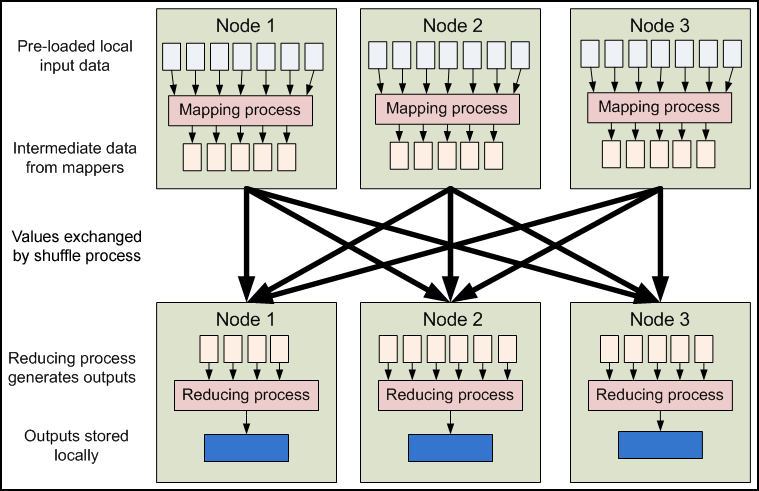
\includegraphics[width=4.0in,
 keepaspectratio=true]{./images/mapreduce-fig1.png}
 % mapreduce-fig1.png: 759x491 pixel, 72dpi, 26.77x17.32 cm, bb=0 0 759 491
 
\end{frame}


%-------------------------------------------------------------------------------
% Hive frame
%-------------------------------------------------------------------------------
\begin{frame}
\frametitle{
\includegraphics[height=0.7in, 
keepaspectratio=false]{./images/hive.png}}

A framework developed by Facebook for data warehousing on top of Hadoop.
\pause
\begin{itemize}
 \item Analysts with strong SQL skill can easily run queries on huge volumes of
data.
  \pause
 \item Query the data using a SQL-like language called HiveQL.
 \pause
 \item Allows custom mappers and reducers when it is inconvenient or
	inefficient to express logic in HiveQL.
\end{itemize}


\end{frame}


%-------------------------------------------------------------------------------
% Big Data Problem: Payment Analysis frame
%-------------------------------------------------------------------------------
\begin{frame}

\frametitle{A Big Data Problem: Payment Analysis}

Predict customer payment behavior based on payment histories.\\
\pause
\begin{itemize}
 \item Requires a batch process to analyze structured and unstructured
datasets.
\pause
 \item Rapid expansion of data size as client base expands.
\pause
 \item Solution should be low-cost, easily manageable, and scalable.\\
\pause
\end{itemize}

\begin{center}
\begin{tabular}{lll}
% use packages: color,colortbl
\rowcolor{lightBlue}
 & \textit{Traditional RDBMS} & \textit{MapReduce}\\
Data size & GB-TBs & TBs-PBs\\
Access & Interactive and batch & Batch\\
Updates & Read/write many times & Write once, read many times\\
Structure & Static Schema & Dynamic Schema\\
Integrity & High & Low\\
Scaling & Nonlinear & Linear
\end{tabular}
\end{center}


\end{frame}


%-------------------------------------------------------------------------------
% Big Data Problem: Payment Analysis frame
%-------------------------------------------------------------------------------
\begin{frame}

\frametitle{A Big Data Problem: Payment Analysis}
\begin{figure}
\centering
 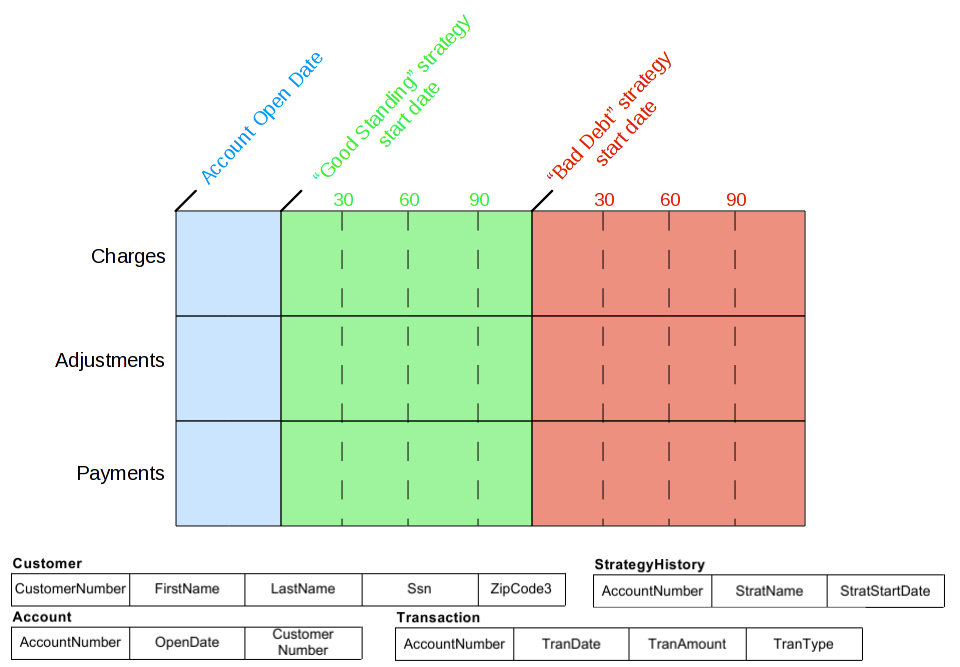
\includegraphics[width=4.0in,
keepaspectratio=true]{./images/payment-analysis.png}
\caption{Aggregate \textcolor{blue}{charges}, \textcolor{blue}{adjustments}, and
\textcolor{blue}{payments} for each account.}
\end{figure}

% \begin{figure}
%  \centering
%  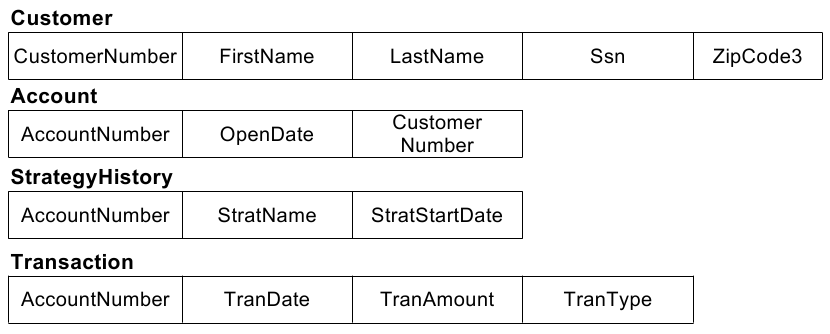
\includegraphics[width=3.5in,keepaspectratio=true]{./images/tuples.png}
%  % tuples.png: 614x242 pixel, 96dpi, 16.24x6.40 cm, bb=0 0 460 181
%  \caption{Tuples defined in company database}
% \end{figure}
% \pause

\end{frame}

%
%-------------------------------------------------------------------------------
% % Big Data frame
%
%-------------------------------------------------------------------------------
% \begin{frame}
% \frametitle{Why Hadoop?}
% 
% 
% 
% \end{center}
% \end{frame}

%-------------------------------------------------------------------------------
% Methods: Requirements frame
%-------------------------------------------------------------------------------
\begin{frame}
\frametitle{Methods: Requirements Phase}

The project requirements will be established as follows:
\begin{enumerate}
\item Meet with consultant.
\pause
\item Clearly outline the details and constraints.
\pause 
\item Work with consultant to verify details and constraints.
\pause 
\item Consistently verify that the requirements are being met and remain
       applicable during all phases of the project.
\end{enumerate}

\end{frame}



%-------------------------------------------------------------------------------
% Methods: Design frame
%-------------------------------------------------------------------------------
\begin{frame}
\frametitle{Methods: Design Phase}
% {\hspace{2.5in}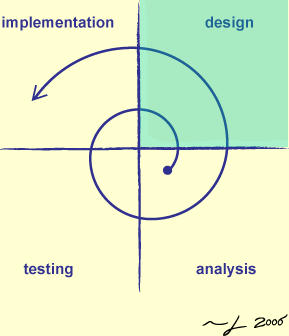
\includegraphics[height=.50in,
%  keepaspectratio=true]{./images/design-phase.png}}
\begin{itemize}
 \item \textbf{Custom writable classes}.
      \begin{enumerate}
       \item \texttt{Customer} - object representing customer tuple.
       \item \texttt{Account} - object representing an account tuple.
       \item \texttt{Transaction} - object representing a transaction tuple.
       \item \texttt{StrategyHistory} - object representing a strategy history
        tuple.
      \end{enumerate}
 \pause
 \item \textbf{MapReduce job flow}. The complexity of the payment analysis
      problem requires several stages of data aggregation to achieve the final
      results. We will need to design the details and algorithms to achieve
      the output for the following jobs.
 \pause
 \item \textbf{Hive dataset structure}. The schema used to store the
       data in HDFS can have profound effects on the efficiency of Hive
       queries. 
\end{itemize}


\end{frame}


%-------------------------------------------------------------------------------
% Methods: Implementation frame
%-------------------------------------------------------------------------------
\begin{frame}
\frametitle{Methods: Implementation Phase}
% {\hspace{2.5in}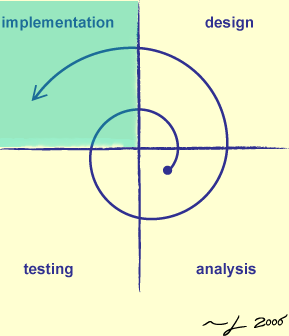
\includegraphics[height=.50in,
%  keepaspectratio=true]{./images/implementation-phase.png}}
\begin{itemize}
  \item Hadoop 0.18 series API and Java 1.6 API
  \pause
  \item Eclipse, MapReduce plug-in, MySQL Workbench
  \pause
  \item Implementation phases:
  \pause
    \begin{enumerate}
      \item MapReduce solution.
      \pause
      \item Sample data generation.
      \pause
      \item Hive solution.
      \pause
      \item Benchmark test cases.
      \pause
    \end{enumerate}
\end{itemize}

\end{frame}


%-------------------------------------------------------------------------------
% Methods: Testing frame
%-------------------------------------------------------------------------------
\begin{frame}
\frametitle{Methods: Testing Phase}
% {\hspace{2.5in}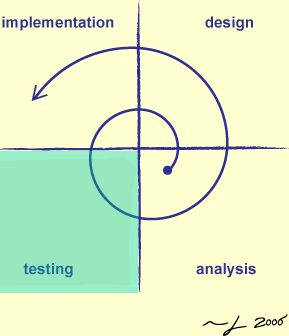
\includegraphics[height=.50in,
%  keepaspectratio=true]{./images/test-phase.png}}

\begin{itemize}

\item Test phase requires the following test cases:
  \begin{itemize}
    \item Read and write accuracy of each {\tt WritableComparable} type.
    \item Output of each MapReduce job and final MapReduce result.
    \item Accuracy of each HiveQL query and final Hive result.
  \end{itemize}

\pause 

\item Most testing during development will occur on a small data set on a
single-node in {\it pseudo-distributed} mode.
\end{itemize}

\end{frame}

%-------------------------------------------------------------------------------
% Methods: Benchmarking frame
%-------------------------------------------------------------------------------
\begin{frame}
\frametitle{Methods: Benchmarking Phase}


\begin{itemize}
 \item Benchmarks include:
  \begin{itemize}
    \pause
   \item \textcolor{blue}{MapReduce} versus \textcolor{blue}{DBMS}: scalability
and performance
    \pause
    \item \textcolor{blue}{Hive} versus \textcolor{blue}{DBMS}: scalability and
performance
   \pause
    \item \textcolor{blue}{MapReduce} versus \textcolor{blue}{Hive}: performance
  \end{itemize}
\pause
\item Considerations:
\pause
  \begin{itemize}
    \item Size of datasets: from 10GB to terabytes. 
    \pause
    \item \textcolor{red}{HDFS cluster design} and \textcolor{red}{DBMS system
specs}: 
    \pause
    \begin{itemize}
      \item A {\it fully-distributed} HDFS cluster running on varied number of
            data nodes (3 to 16).
      \pause
      \item The estimated cost of the DBMS system and HDFS cluster will be
            comparable for comparison tests.
    \end{itemize}

  \end{itemize}
\end{itemize}
\end{frame}
%-------------------------------------------------------------------------------
% Project Schedule frame
%-------------------------------------------------------------------------------
\begin{frame}[fragile,shrink=12]
\begin{center}
\frametitle{Project Schedule}

\begin{tabular}{ | l || p{3.5in} | }\hline
 December 2010 & - Meet with consultant to define problem.\\\hline
  January 2011 & - Obtain specification documents and start application design
     phase.\\\hline
 February 2011 & - Solidify application requirements and design.\\
        \hfill & - Begin implementation and test phases of MapReduce
                 solution.\\\hline
    March 2011 & - Finalize MapReduce solution.\\
        \hfill & - Begin implementation phase of sample data generation.\\\hline
    April 2011 & - Use sample data to compare MapReduce implementation to MySQL
                 solution.\\
        \hfill & - Begin implementation and test phases of Hive solution.\\
        \hfill &-  Write report sections for MapReduce solution.\\\hline
      May 2011 & - Finalize Hive solution.\\
        \hfill & - Use sample data to compare Hive implementation to MapReduce  
                 and MySQL implementations.\\
        \hfill & - Write report sections for Hive solution.\\
        \hfill & - Finalize report.\\\hline
\end{tabular}

\end{center}
\end{frame}


\end{document}